\chapter{Architettura Hardware dello strumento}
\label{capitolo3}
\thispagestyle{empty}

\textit{In questo Capitolo verrà descritta l'architettura hardware dello strumento realizzato. Prima verrà analizzata brevemente la parte analogica dello strumento. Successivamente verrà descritta la parte di conversione analogico-digitale e digitale-analogico soffermandoci prima sulle architetture dei convertitori presenti in letteratura e poi su quelle presenti nello strumento. Infine verrà presentata la parte digitale motivando la scelta dell'uso di una scheda di prototipazione contenente FPGA e microcontrollore.}

\section{Struttura complessiva dello strumento}
Lo strumento di misura progettato in questo elaborato è un misuratore \textit{contactless} di distanza. Lo scopo è realizzare un sistema \textit{embedded} in grado di gestire in modo autonomo tutta la misura, dal controllo della sorgente laser all'acquisizione ed elaborazione del segnale interferometrico.

Per sistema \textit{embedded}, si intende un sistema di elaborazione progettato appositamente per una specifica applicazione (\textit{special purpose}). Come già introdotto, l'applicazione in questione è la misura di distanza. 

Il principio fisico per il quale è possibile effettuare una misura è stato descritto nel Capitolo \ref{capitolo2}.
\begin{figure}  
  \begin{center}
  %%TODO Cap3: Foto finale dello strumento
    %\includegraphics[scale=0.5]{}
    \caption{Risultato finale del misuratore realizzato}
    \label{fotorisfin}
  \end{center}
\end{figure}\\
La Figura \ref{fotorisfin} mostra il risultato finale del misuratore progettato e realizzato per questo lavoro di Tesi. Dalla figura si possono distinguere le tre parti principali che compongono lo strumento:
\begin{itemize}
	\item \underline{Parte analogica}: La parte analogica è costituita da una sezione ottica e una sezione analogica. La sezione ottica è composta dal package della sorgente laser, che comprende laser, fotodiodo e lente collimatrice. La sezione analogica comprende il circuito di alimentazione del laser e gli stadi di condizionamento e amplificazione del segnale interferometrico generato dal fotodiodo.
	\item \underline{Parte di conversione}: La parte di conversione è formata da due sezioni: la sezione di conversione analogico-digitale (ADC) e la sezione di conversione digitale-analogico (DAC). La prima sezione provvede ad effettuare la conversione analogico-digitale del segnale interferometrico in uscita dalla parte analogica. Mentre, la seconda sezione effettua la conversione digitale-analogica dal segnale di modulazione del laser in uscita dalla parte digitale.
	\item \underline{Parte digitale}: La parte digitale è costituta da un dispositivo \textit{embedded} di prototipazione composto da un microprocessore e un FPGA. I compiti principali della parte digitale sono la generazione del segnale di modulazione del laser, l'elaborazione del segnale interferometrico per l'estrazione della frequenza di frangia e il calcolo della misura di distanza. Un computer è collegato con la parte digitale tramite connessione \textit{Ethernet}, attraverso questo collegamento è possibile la comunicazione con gli elementi programmabili del sistema.
\end{itemize}
\begin{figure}  
  \begin{center}
    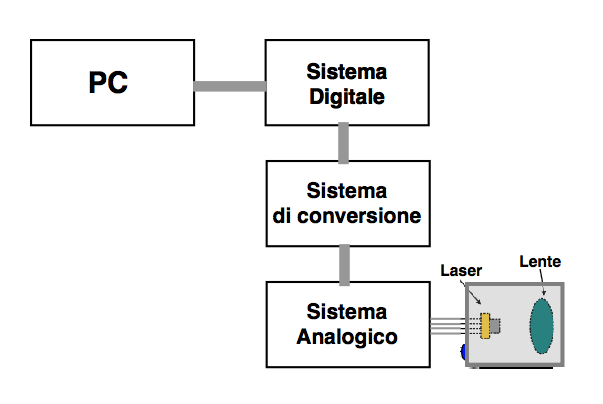
\includegraphics[scale=0.5]{cap3/archgen}
    \caption{Schema a blocchi dell'architettura complessiva del misuratore}
    \label{archgen}
  \end{center}
\end{figure}

L'architettura complessiva del sistema progettato è schematizzata in Figura \ref{archgen}. La Figura mostra lo schema concettuale dello strumento, evidenziando le singoli parti e le connessioni fra quest'ultime.

Nei paragrafi successivi verrà fornita un'analisi dettagliata delle singoli parti dello strumento.

\section{Parte analogica}
La parte analogica è formata da due sotto-sistemi:
\begin{enumerate}
	\item Sistema ottico e sorgente laser
	\item Circuito di interfacciamento con il modulo laser
\end{enumerate}

\subsection{Sistema ottico e sorgente laser}
In lavori precedenti sono state provate diverse sorgenti~\cite{thesispallsilv}~\cite{thesisstorti}. Tra queste è stato scelto il modulo laser \textit{WLSD-1550-020m-1-PD}.
\begin{figure}  
  \begin{center}
    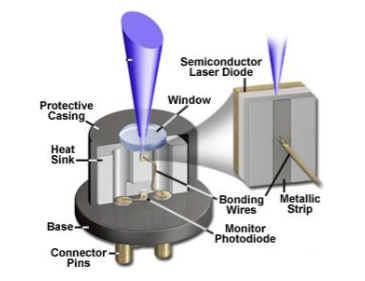
\includegraphics[scale=0.5]{cap3/laserwave}
    \caption{Struttura del dispositivo \textit{WLSD-1550-020m-1-PD}}
    \label{laserwave}
  \end{center}
\end{figure}

Si tratta di una sorgente laser di tipo DFB (\textit{Distributed FeedBack}) prodotta dalla \textit{Wavespectrum}, la cui struttura è mostrata in Figura \ref{laserwave}. Essa emette ad una lunghezza d'onda di $1550nm$.

La sorgente è allineata alla lente per la collimazione, questi due componenti alloggiano in un supporto di alluminio. La lente, codice prodotto \textit{C230TMD-C} realizzata da \textit{Thorlabs}, ha la funzione di raccogliere tutto il fascio laser della sorgente focalizzandolo a piacere. \'E possibile infatti regolarne la posizione avvitandola o svitandola.

Di seguito vengono riassunti i punti chiave che hanno portato alla scelta di tale sorgente laser:
\begin{itemize}
	\item Possiede un buon rapporto segnale/rumore
	\item \'E facile modularne la lunghezza d'onda
	\item Essendo un laser DFB riflette solo una banda ristretta di lunghezze d'onda
	\item Ha un costo accessibile
	\item Appartiene alla classe di sicurezza $1$
	\item Ha una debole riflettività dello specchio permettendo così una forte sensibilità alla retroiniezione
\end{itemize}

Tale sorgente però, emettendo nel non visibile, rende complicati i processi di allineamento.
\begin{figure}  
  \begin{center}
    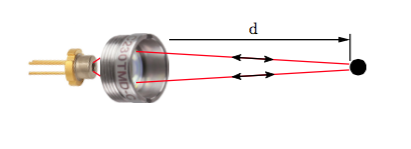
\includegraphics[scale=0.5]{cap3/sistottico}
    \caption{Sistema ottico con laser e lente}
    \label{sistottico}
  \end{center}
\end{figure}
In figura \ref{sistottico} è mostrato il sistema ottico senza supporto. Il bersaglio è schematizzato con un pallino nero e $d$ è la distanza misurata.

\subsection{Circuito di interfacciamento}
Come ampiamente descritto nel Capitolo precedente, è necessario generare una corrente di modulazione sovrapposta a quella di polarizzazione per il diodo laser. Per tale motivo, questo circuito si occupa dell'elaborazione dei segnali analogici, rispettivamente della corrente di pilotaggio del laser e della corrente di uscita dal fotodiodo.
\begin{figure}  
  \begin{center}
    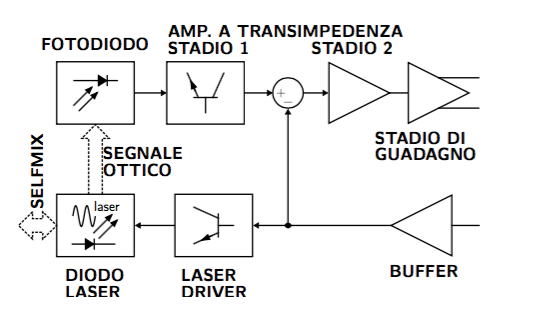
\includegraphics[scale=0.5]{cap3/circanalog}
    \caption{Schema a blocchi del circuito di interfacciamento}
    \label{circanalog}
  \end{center}
\end{figure}

Lo schema logico del circuito è mostrato in Figura \ref{circanalog}. 

Il segnale di modulazione proveniente dalla parte di conversione attraversa un circuito di filtraggio e viene convertito in corrente (corrente di pilotaggio del laser).
Il segnale di corrente dovuto all'effetto interferometrico è minore di $2 \mu A$ , molto più ampio invece è quello associato alla modulazione (circa $1mA$). Per poter estrarre solamente il segnale interferometrico si effettua quindi una differenza del segnale totale rilevato con quello di modulazione del laser. Infine, il risultato della differenza è ulteriormente amplificato e reso disponibile alla parte di conversione in formato differenziale.

Una descrizione più dettagliata della parte analogica e dell'attività di progetto del sistema è trattata nel lavoro di tesi sviluppato dal laureando Samuele Disegna con cui abbiamo collaborato~\cite{thesissmldis}.

\section{Parte di Conversione}
La scheda utilizzata per la parte di conversione del misuratore è la \textit{SCO Board}, progettata e prodotta nel laboratorio di "Misure Ottiche ed Elettroniche - MOLES" del Politecnico di Milano. Anch'essa è stata progetta e realizzata da Samuele Disegna nel contesto del suo lavoro di tesi.

Essa possiede due interfacce di conversione: un'interfaccia Analogico-Digitale (AD), che riceve in ingresso il segnale interferometrico in arrivo dalla sorgente laser, e un'interfaccia Digitale-Analogica (DA), che converte il segnale digitale di modulazione in arrivo dalla scheda di prototipazione. Le conversioni AD e DA vengono svolte in parallelo.

\begin{figure}  
  \begin{center}
    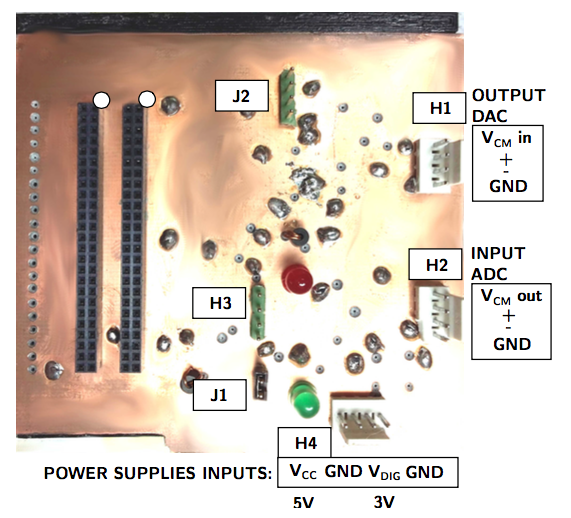
\includegraphics[scale=0.5]{cap3/scoboardfoto}
    \caption{Foto della scheda di conversione \textit{SCO Board} e identificazione delle connessioni}
    \label{scoboardfoto}
  \end{center}
\end{figure}

\begin{figure}  
  \begin{center}
    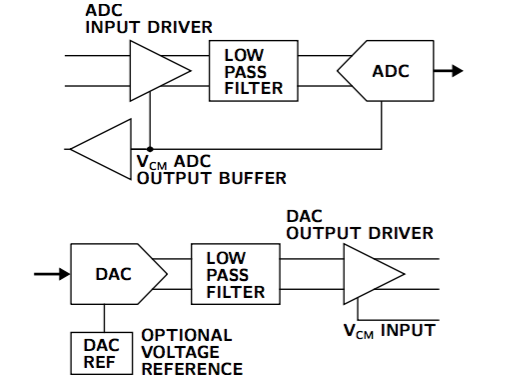
\includegraphics[scale=0.5]{cap3/scoboardschema}
    \caption{Schema a blocchi del sistema di conversione A/D - D/A, \textit{SCO Board}}
    \label{scoboardschema}
  \end{center}
\end{figure}

Le specifiche fornite per la frequenza massima di campionamento dei segnali sono $50MS/s$ con $12$ bit di quantizzazione, essi garantiscono di avere una buona dinamica di misura della distanza e una buona dinamica di ampiezza del segnale misurato con rumore di quantizzazione trascurabile. In Figura \ref{scoboardfoto} e \ref{scoboardschema} sono mostrate rispettivamente la \textit{SCO Board} e il relativo schema a blocchi del circuito.

I due amplificatori operazionali completamente differenziali si occupano della gestione dei segnali analogici. Uno pilota l'uscita differenziale corrispondente al DAC e porta la dinamica di uscita a $1V_{pp}$, l'altro prepara il segnale di ingresso differenziale per il campionamento. I filtri passa basso svolgono la funzione di antialiasing per l'ADC e di ricostruzione del segnale del DAC.

I convertitori presenti sulla \textit{SCO Board} e le loro caratteristiche fondamentali verranno descritte in dettaglio nei paragrafi successivi.

Invece, una descrizione più dettagliata del circuito è fornita in letteratura~\cite{thesissmldis}.

\subsection{Convertitori}
I convertitori Digitale-Analogico (DAC) e Analogico-Digitale (ADC) fanno parte della famiglia dei convertitori dati (\textit{Data Converters}).

Le caratteristiche fondamentali di un convertitore dati sono:
\begin{itemize}
	\item \underline{Risoluzione}: Descrive il numero di valori (livelli di quantizzazione) che il convertitore riesce a distinguere. L'unità di misura è il numero di bit $n$. I livelli di quantizzazione $N$ sono definiti come:
	\begin{equation}
		N=2^n
	\end{equation}
	\item \underline{Dinamica}: Descrive la massima ampiezza del segnale analogico. L'unità di misura è il volt $[V]$.
	\item \underline{Tempo di conversione}: Indica il tempo impiegato dal convertitore per eseguire la conversione. I tempi impiegati per la conversione differiscono notevolmente a seconda della tipologia di convertitore utilizzato, anche se, in generale, la conversione DA è più veloce dell'operazione inversa. Di solito è più conveniente specificare il numero di campioni che possono essere convertiti in un secondo, piuttosto che il tempo di conversione. Tale grandezza è chiamata frequenza di campionamento (o \textit{sampling rate}) e si esprime in Hertz $[Hz]$ o campioni per secondo $[Sa/s]$.
\end{itemize}

Come descritto nel paragrafo precedente, le specifiche fornite per la frequenza massima di campionamento dei segnali sono $50MS/s$ con $12$ bit di risoluzione.

Nei paragrafi successivi verrà trattato lo stato dell'arte dei convertitori dati e verranno descritte le architetture dei convertitori presenti sulla scheda di conversione utilizzata.

\subsubsection{Convertitore DAC}
Il processo di ricostruzione di un segnale analogico consiste nel prelevare valori digitali e convertirli nei loro equivalenti analogici. Questa operazione è svolta dal convertitore Digitale-Analogico (DAC)~\cite{storeyelet}.

\begin{figure}  
  \begin{center}
    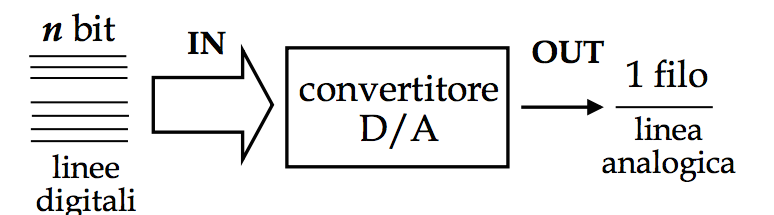
\includegraphics[scale=0.35]{cap3/dac}
    \caption{Schema di funzionamento di un convertitore Digitale-Analogico (DAC)}
    \label{dac}
  \end{center}
\end{figure}

\paragraph{Architetture DAC}
Esistono due architetture comuni di DAC:
\begin{enumerate}
	\item A resistori pesati (o \textit{Binary-weighted resistor})
	\item A scala R-2R (o \textit{R-2R resistor chain})
\end{enumerate}
\begin{figure}  
  \begin{center}
    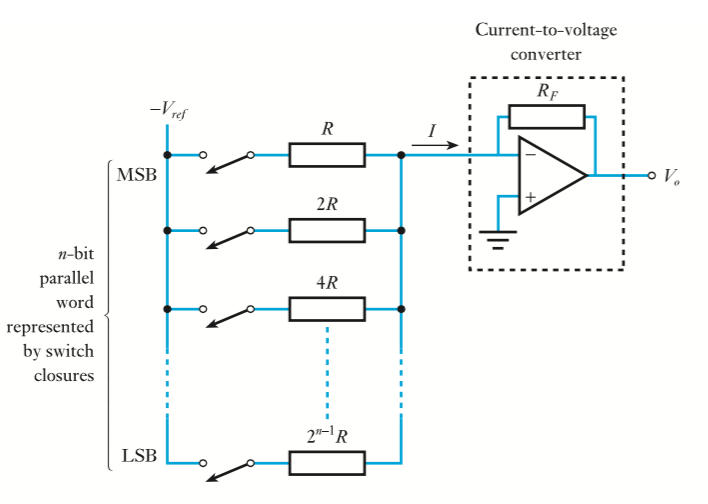
\includegraphics[scale=0.4]{cap3/bwdac}
    \caption{Struttura circuitale di un DAC a resistori pesati}
    \label{bwdac}
  \end{center}
\end{figure}
\subparagraph{\textbf{DAC a resistori pesati}} La Figura \ref{bwdac} illustra lo schema circuitale di un generico DAC a resistori pesati a n bit.
Il circuito, mostrato in figura, è costituito da $n$ interruttori pilotati dagli $n$ bit della parola in ingresso, $n$ resistori pesati su un valore di riferimento $R$, e un convertitore corrente-tensione invertente.

Ogni ingresso controlla un interruttore (\textit{switch}) che collega un resistore a un riferimento di tensione. Quando il generico bit dell'ingresso è a $1$ il corrispondente interruttore viene collegato al riferimento di tensione $-V_{ref}$, mentre quando il bit è a $0$ l'interruttore viene collegato a massa ($0 V$).

Data la corrente passante nell' $i$-esimo interruttore controllato dal bit $b_i$ della parola:
\begin{equation}
	I_i=-\frac{V_{ref}}{2^{(n-1)-i}R}b_i = -\frac{V_{ref}}{2^{(n-1)}R}2^ib_i
\end{equation}
si ricava la corrente complessiva della rete di resistori pesati:
\begin{equation}
	I = \sum_{k=1}^{n-1} I_k = -\frac{V_{ref}}{2^{(n-1)}R} \sum_{k=1}^{n-1} 2^k b_k 
\end{equation}
Infine, per effetto del convertitore corrente-tensione si ha:
\begin{equation}
	V_0 = -R_f I
\end{equation}
dove $R_f$ è il resistore di feedback. L'equazione definisce la relazione ingresso-uscita del DAC.

I vantaggi di questa configurazione sono la semplicità di realizzazione del circuito e l'utilizzo di un ristretto numero di resistenze ($n$ bit, $n$ resistenze). Per tale motivo le risoluzioni tipiche per questo metodo sono inferiori ai $10$ bit.

Lo svantaggio maggiore è la difficoltà nel realizzare resistenze con valori differenti e perfettamente calibrati, in modo tale che i loro rapporti tra esse siano precisi.
Per tale motivo questa configurazione è tuttavia poco usata nella pratica.

\subparagraph{\textbf{DAC a scala R-2R}}
Il DAC a resistenze pesate visto nella paragrafo precedente presenta problemi di realizzazione e di funzionamento, dovuti sostanzialmente all'uso di resistori molto differenti fra di loro. Questi problemi possono essere risolti usando un'altra architettura circuitale: il DAC a scala R-2R.

La figura \ref{r2rdac} illustra lo schema circuitale di un generico DAC a scala R-2R a $n$ bit.
Il circuito, mostrato in figura, è costituito da $n$ interruttori pilotati dagli $n$ bit della parola in ingresso, $n$ resistori e un convertitore corrente-tensione invertente. 

La differenza in questo caso è che tutti i resistori collegati agli interruttori hanno lo stesso valore $2R$. Inoltre, l'estremità di ogni resistore è collegata ad una catena di resistenze che va dall'ingresso invertente del convertitore corrente-tensione a massa.
\begin{figure}  
  \begin{center}
    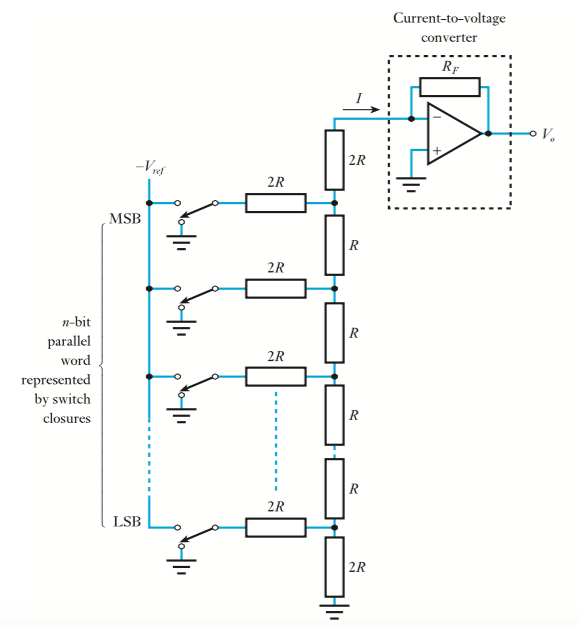
\includegraphics[scale=0.4]{cap3/r2rdac}
    \caption{Struttura circuitale di un DAC a scala R-2R}
    \label{r2rdac}
  \end{center}
\end{figure}

Il circuito è realizzato in modo tale che le correnti che fluiscono attraverso i resistori collegati agli interruttori vedano una resistenza $2R$ guardando in entrambe le direzioni lungo la catena delle resistenze. Pertanto, metà della corrente andrà in ciascuna direzione. 

Allo stesso modo, le correnti che scorrono lungo la catena vedono resistenze uguali in entrambe le direzioni e ad ogni nodo vengono nuovamente divise.

Riassumendo, ciascun interruttore contribuisce con metà della corrente fornita dall'interruttore sopra, e tale corrente viene ripetutamente dimezzata da ogni nodo incontrato nel percorso verso l'amplificatore operazionale.

Pertanto, le correnti generate dagli interruttori sono pesate, come nel metodo precedente, ma senza l'uso di un ampio intervallo di valori di resistenza. Dunque questa architettura presenta il vantaggio di utilizzare solo due valori resistivi risultando più facile da realizzare.

I tempi di conversione dei metodi precedentemente descritti sono simili. Essi sono determinati dal tempo impiegato dagli interruttori per cambiare stato e dal tempo di risposta dell'amplificatore operazionale. In generale il tempo di conversione cresce all'aumentare della risoluzione. Un DAC a $8$ bit per applicazioni generiche (\textit{general-purpose}) possiede tempi di conversione compresi tra i $100ns$ e $1ms$, mentre un convertitore a $16$ bit può avere un tempo di conversione nell'ordine dei microsecondi.

Per applicazioni specifiche, come nel caso del misuratore oggetto di questo lavoro di tesi, sono necessari convertitori ad alta velocità con tempi di conversione nell'ordine dei nanosecondi. Per raggiungere tali prestazioni l'uso di una singola architettura non basta, pertanto è necessario combinare due o più architetture allo scopo di raggiungere le prestazioni richieste. Il procedimento è noto come "segmentazione" e questa  architettura è chiamata "DAC segmentato” (\textit{Segmented DAC}). 

\paragraph{Convertitore DAC presente sulla scheda di conversione}
Il convertitore presente sulla scheda di conversione \textit{SCO Board} è il \textit{DAC902}. \'E un convertitore DAC Segmentato prodotto dalla \textit{Texas Instruments} con una risoluzione di $12$ bit e una velocità di campionamento massima pari a $165MHz$.
Tale architettura rispetta pienamente le specifiche prefissate con una frequenza di campionamento massima ben superiore a quella richiesta.

Questo convertitore utilizza la tecnica della somma di correnti vista nelle precedenti due architetture, ma al contrario di quest'ultime i generatori di corrente sono implementati con transistor PMOS invece che con resistori e tensioni di riferimento.
\begin{figure}  
  \begin{center}
    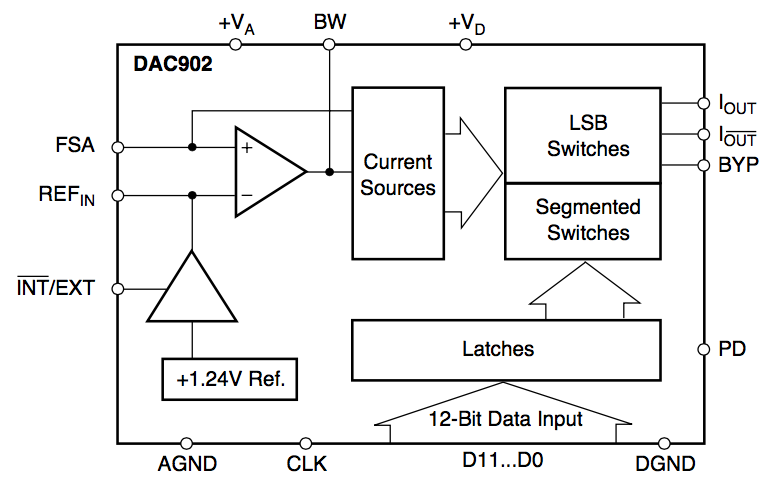
\includegraphics[scale=0.3]{cap3/schemadac902}
    \caption{Schema a Blocchi interno del DAC - DAC902}
    \label{schemadac902}
  \end{center}
\end{figure}
L'architettura segmentata utilizzata in questo integrato sfrutta due architetture: un DAC gestisce i bit più significativi (MSB) e un altro gestisce i bit meno significativi (LSB). Lo schema a blocchi è mostrato in figura \ref{schemadac902}.

Una descrizione più dettagliata dell'integrato è fornita sul sito del costruttore~\cite{sitedac902}.

\subsubsection{Convertitore ADC}
Il processo di campionamento di un segnale analogico consiste nel prelevare una lettura istantanea della sua grandezza e di convertirla in una forma digitale. Questa operazione è svolta dal convertitore Analogico-Digitale (ADC)~\cite{storeyelet}.
\begin{figure}  
  \begin{center}
    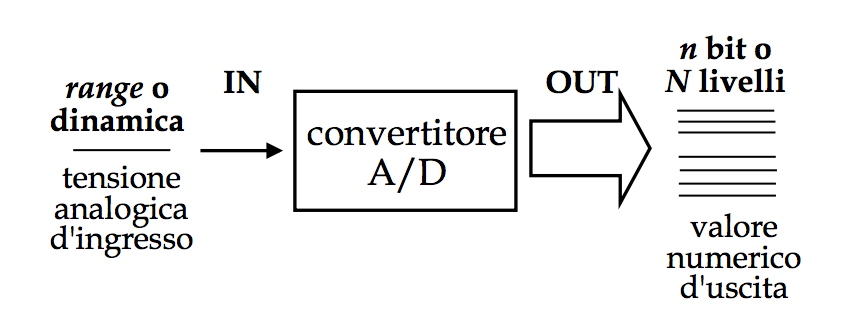
\includegraphics[scale=0.35]{cap3/adc}
    \caption{Schema di funzionamento di un convertitore Analogico-Digitale (ADC)}
    \label{adc}
  \end{center}
\end{figure}

\paragraph{Architetture ADC}
Esistono cinque architetture comuni di ADC:
\begin{enumerate}
	\item A conteggio (\textit{Counter})
	\item Ad approssimazioni successive (\textit{Successive Approximation})
	\item A Doppia rampa (\textit{Dual Slope})
	\item Flash
	\item Pipeline
\end{enumerate}

\subparagraph{\textbf{ADC a conteggio}}
\begin{figure}  
  \begin{center}
    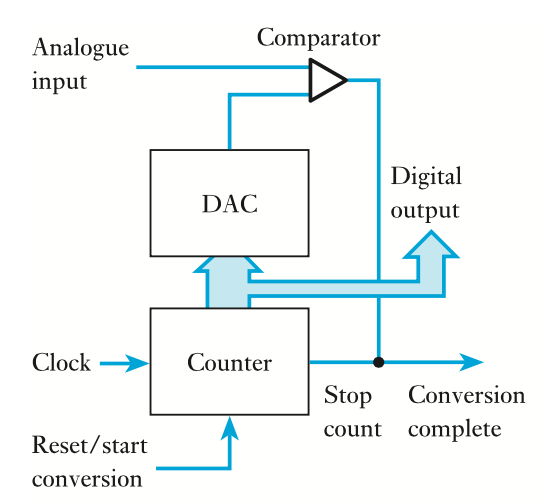
\includegraphics[scale=0.35]{cap3/adccounter}
    \caption{Schema di funzionamento di un ADC a conteggio}
    \label{adccounter}
  \end{center}
\end{figure}
L'ADC a conteggio è una delle forme più semplici di convertitore ADC. Lo schema di funzionamento è mostrato in Figura \ref{adccounter}.

Il cuore dell'architettura è costituito da un contatore incrementale. La conversione viene effettuata iniziando un nuovo conteggio a partire da zero. L'uscita del contatore viene convertita in analogico dal DAC e quindi confrontata con la tensione di ingresso mediante un comparatore. Un comparatore è un dispositivo che produce un'uscita booleana a seconda di quale dei due ingressi è maggiore. Quando il valore prodotto dal DAC supera la tensione di ingresso, il conteggio viene bloccato e tale valore rappresenta il valore di tensione di uscita.

Questo metodo è di semplice realizzazione, ma i principali difetti sono la lentezza e il tempo di conversione non costante. Per un ADC a $n$ bit, la conversione può richiedere nel caso pessimo $2^{n-1}$ cicli di clock. Il tempo di conversione è solitamente nell'ordine dei millisecondi (ca. $500 Sa/s$).

Una versione migliorata dell'ADC a conteggio è l'ADC a inseguimento (\textit{servo ADC}): il contatore incrementale viene sostituito con un contatore incrementale/decrementale. Pertanto, l'uscita del comparatore è utilizzata come segnale di comando del contatore, forzando il contatore a "inseguire" segnale di ingresso analogico. Esso risulta più veloce dell'ADC a conteggio, a condizione che i valori di tensione da convertire siano abbastanza vicini fra loro.

%%TODO Cap3: Figura confronto servo adc - counter adc 
\subparagraph{\textbf{ADC a conteggio}}
\begin{figure}  
  \begin{center}
    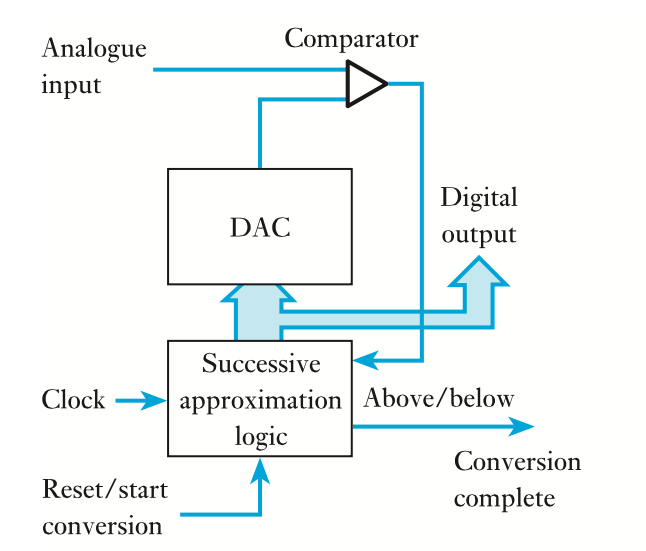
\includegraphics[scale=0.35]{cap3/adcsar}
    \caption{ADC ad approssimazioni successive}
    \label{adcsar}
  \end{center}
\end{figure}
L'ADC ad approssimazioni successive è basato su una logica di controllo costituita da un registro ad approssimazioni successive chiamato SAR (\textit{Successive Approximation Register}). Lo schema di funzionamento è mostrato in Figura \ref{adcsar}.

Questa architettura è simile a quella dell'ADC a conteggio, fatta eccezione che il semplice contatore incrementale è sostituito dalla logica di controllo SAR. Come negli ADC a conteggio, la conversione avviene confrontando l'uscita di un convertitore DAC con la tensione in ingresso.

Il DAC viene comandato dalla parola digitale prodotta dalla logica di controllo. Inizialmente, tutti i bit della parola digitale sono impostati a 0 mentre il bit più significativo (MSB, \textit{Most Significant Bit}) è impostato a $1$. Questo valore viene convertito e confrontato con il segnale di ingresso analogico utilizzando il comparatore ed il risultato del comparatore viene inviato al SAR. Se la tensione di ingresso è maggiore della parola digitale corrente, il SAR mantiene l'MSB a 1 e carica un altro 1 nel bit immediatamente successivo, altrimenti pone l'MSB a 0 e carica sempre un 1 nel bit immediatamente successivo. I passi appena descritti vengono reiterati fino al bit meno significativo (LSB, \textit{Least Significant Bit}). Il metodo appena descritto è chiamato metodo di \textit{bisezione}.

Il tempo di conversione dell'ADC è costante qualunque sia il valore della tensione in ingresso. Indicando con $T_{ck}$ il periodo del clock e con $n$ bit il numero di bit del convertitore, il tempo di conversione $T_{conv}$ è pari a:
\begin{equation}
	T_{conv}=nT_{ck}
\end{equation}

Questa architettura raggiunge velocità di conversione migliori dell'ADC a conteggio, perdendo però in semplicità di realizzazione.

Solitamente i convertitori SAR possiedono risoluzioni comprese tra gli $8$ e i $12$ bit con tempi di conversione nell'ordine dei microsecondi ($50 \div 400 KSa/s$).

\subparagraph{\textbf{ADC a Doppia rampa}}
\begin{figure}  
  \begin{center}
    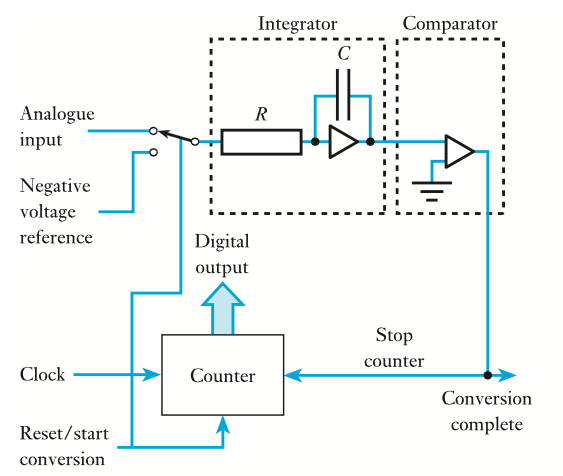
\includegraphics[scale=0.35]{cap3/adcdoppiarampa}
    \caption{Schema di funzionamento di un ADC a doppia rampa}
    \label{adcdoppiarampa}
  \end{center}
\end{figure}
L'ADC a doppia rampa è un convertitore basato sull'utilizzo di un integratore. Lo schema di funzionamento è mostrato in Figura \ref{adcdoppiarampa}.

L'amplificatore operazionale integra il segnale di ingresso per un determinato periodo di tempo, producendo una carica sul condensatore proporzionale alla tensione di ingresso. L'integratore viene poi collegato ad un riferimento di tensione negativo che permette di scaricare il condensatore ad una velocità costante.

Il tempo impiegato per scaricare il condensatore viene misurato da un contatore. Il tempo di scarica è proporzionale alla quantità di carica presente nel condensatore e quindi alla tensione di ingresso. Tale conteggio corrisponde al valore digitale prodotto in uscita.

Questa tecnica si utilizza in quelle applicazioni in cui il segnale da convertire varia lentamente nel tempo, privilegiando la precisione rispetto alla rapidità di conversione. Con questi convertitori è possibile raggiungere risoluzioni maggiori di $20$ bit portando però il tempo di conversione sull'ordine dei secondi ($10 \div 100 Sa/s$).

\subparagraph{\textbf{ADC Flash}}
\begin{figure}  
  \begin{center}
    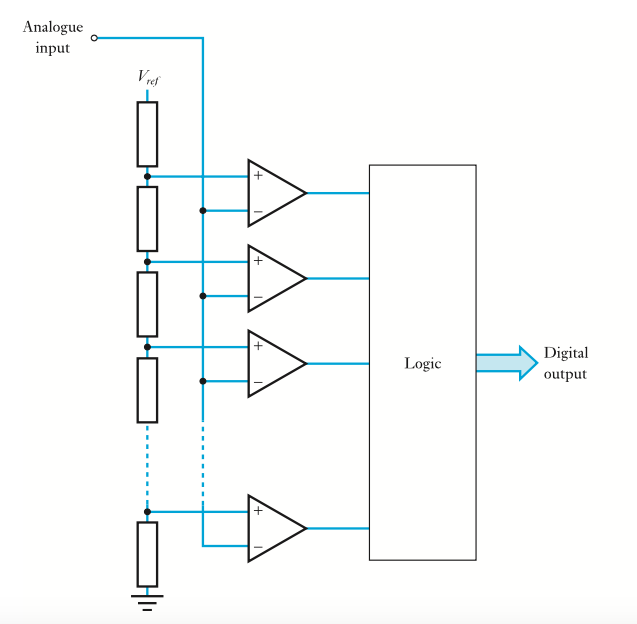
\includegraphics[scale=0.35]{cap3/adcflash}
    \caption{Schema di funzionamento di un ADC Flash}
    \label{adcflash}
  \end{center}
\end{figure}
L'ADC Flash è basato sull'utilizzo di compratori in parallelo. Lo schema di funzionamento è mostrato in Figura \ref{adcflash}.

Il segnale di ingresso di un ADC Flash a $n$ bit, viene confrontato con $2^n$ tensioni di riferimento, tipicamente generate con una stringa resistiva realizzata con $2^n$ resistori, tramite $2^n$ comparatori. Il risultato è che tutti i comparatori che hanno tensioni superiori alla tensione di ingresso produrranno un uscita di tensione positiva, mentre quelli collegati a tensioni al di sotto della tensione di ingresso produrranno tensioni di senso opposto. La logica combinatoria viene quindi utilizzata per determinare il valore digitale di uscita.

Il grosso vantaggio di questa tecnica è la velocità di conversione, essa permette di raggiungere tempi di conversione nell'ordine dei nanosecondi (fino a $40 GSa/s$): è la tecnica ADC più veloce. 

Lo svantaggio è l'alto costo di realizzazione ($n$ bit implica $2^n$ comparatori). Pertanto, le risoluzioni tipiche sono di $8$ bit.

\subparagraph{\textbf{ADC Pipeline}}
\begin{figure}  
  \begin{center}
    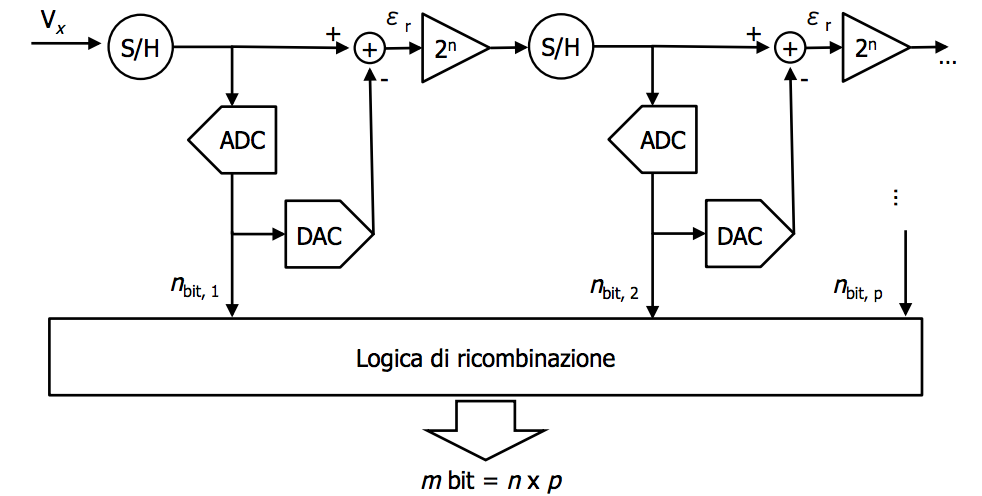
\includegraphics[scale=0.35]{cap3/adcpipeline}
    \caption{Schema di funzionamento di un ADC Pipeline }
    \label{adcpipeline}
  \end{center}
\end{figure}
L'ADC Pipeline è un convertitore che sfrutta il principio della pipeline. Lo schema di funzionamento è mostrato in Figura \ref{adcpipeline}.

Una pipeline è un insieme di stadi di elaborazione connessi in serie, in cui l'uscita di un elemento è l'ingresso del successivo. Gli stadi sono identici, quindi è sufficiente spiegare il funzionamento del primo per comprendere il funzionamento di tutta l'architettura.

Il segnale analogico d'ingresso viene convertito da un ADC SAR a $n$ bit. Il segnale digitale così prodotto costituisce l'uscita dello stadio. Il segnale ottenuto dal SAR, oltre che essere l'uscita dello stadio, costituisce l'ingresso di un DAC, che fornisce in uscita nuovamente un segnale analogico, che però differisce da quello originale in quanto affetto da errore di quantizzazione introdotto dal SAR.

Il campione così ottenuto va in ingresso a un sommatore che ne fa la differenza col segnale analogico originale, ottenendo così come risultato l'errore di quantizzazione. Successivamente l'errore di quantizzazione va in ingresso a un amplificatore di guadagno $2^n$, in modo da poter sfruttare al massimo l'intervallo di conversione del ADC SAR. Infine, gli stadi successivi al primo convertono l'errore di quantizzazione. I bit ottenuti in uscita dai diversi stadi vengono poi riallineati tramite opportuni registri, in modo da costituire la parola digitale di uscita. 

La risoluzione di un convertitore Pipeline risulta limitata dalla precisione dei convertitori AD e DA presenti nell'architettura. La massima risoluzione ottenibile si aggira da un minimo di $8$ bit a un massimo di $24$ bit  con velocità di conversione sull'ordine dei nanosecondi ($1 \div 200 MSa/s$). 

\paragraph{Convertitore ADC presente sulla scheda di conversione}
Il convertitore presente sulla scheda di conversione \textit{SCO Board} è l'\textit{ADS807}. \'E un convertitore ADC Pipeline prodotto dalla \textit{Texas Instruments} con una risoluzione di $12$ bit e una velocità di campionamento massima pari a $53MHz$. Tale convertitore rispetta pienamente le specifiche prefissate.

\begin{figure}  
  \begin{center}
    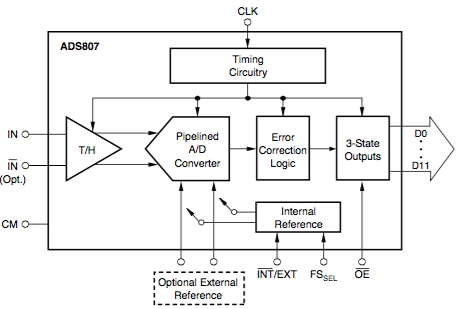
\includegraphics[scale=0.5]{cap3/ads807schema}
    \caption{Schema di funzionamento del ADS807}
    \label{ads807schema}
  \end{center}
\end{figure}

La figura \ref{ads807schema} mostra lo schema a blocchi interno del \textit{ADS807}.
Il circuito è costituito da quattro componenti principali:
\begin{itemize}
	\item \underline{Circuito di Track \& Hold}: L'ingresso analogico consiste in un circuito differenziale di \textit{Track \& Hold}. Tale circuito è utilizzato per mantenere il segnale campionato costante durante tutto il periodo di conversione. A differenza di un \textit{Sample \& Hold}, il \textit{Track \& Hold} trascorre la maggior parte del tempo seguendo l'ingresso ed è posto in modo hold solo per un breve intervallo. Nei sistemi di acquisizione che operano ad elevate velocità, come in questo caso (superiori a $1MHz$), i termini \textit{Sample \& Hold} e \textit{Track \& Hold} perdono la loro distinzione. 
\end{itemize}


\section{Parte digitale}

\subsection{Scheda di prototipazione utilizzata}

\subsection{FPGA}

\subsubsection{Storia delle FPGA}

\subsubsection{Tecniche di implementazione delle FPGA}

\subsection{Xilinx Spartan-6 LX45}

\subsubsection{Utilizzo FPGA}

\subsection{Microcontrollore}

\subsubsection{Architettura PowerPC}
